\chapter{Introduction}
\label{chap:intro}
% 1. Introduction ~3 pages: What is a blazar, what is polarization, how we measure polarization and how it could be improved, what we can learn about blazars with polarization.

Measuring X-ray polarization has been a major goal in astrophysics for the last 40 years. X-ray polarization measurements offer rich opportunities to probe the magnetic field topology and emission physics of high energy astrophysical sources, such as accreting black holes and astrophysical jets \citep{krawczynski_using_2019, weisskopf_overview_2018}. 
The recent development of photoelectron tracking detectors \citep{bellazzini_novel_2003} has greatly improved the prospects of doing so. The gas pixel detector (GPD) \citep{bellazzini_sealed_2007} has brought soft X-ray polarimetry (1-10 keV) to the PolarLight CubeSat test \citep{feng_x-ray_2020}, the scheduled NASA IXPE mission \citep{sgro_imaging_2019}, and the potential Chinese mission, eXTP \citep{zhang_extp_2017}. 

Deep neural networks have achieved state-of-the-art performance on a wide variety of machine learning tasks and are becoming increasingly popular in domains such as speech recognition \citep{graves_connectionist_2006}, natural language processing \citep{young_recent_2018}, bioinformatics \citep{tang_recent_2019} and especially computer vision \citep{krizhevsky_imagenet_2012}. Going from track images to emission angle estimates can be classified as a computer vision problem, so it is not surprising that neural networks would be well suited to track reconstruction. The Cherenkov Telescope Array (CTA) \citep{brill_investigating_2019} team have applied related deep learning methods to differentiate between cosmic rays and gamma rays. Notably they also have to deal with a hexagonal pixel grid, also found in imaging X-ray polarimeters. The IceCube collaboration has begun the use of graph neural networks to identify 3D neutrino tracks with great success \citep{choma_graph_2018}. 
This section briefly covers deep neural network and machine learning concepts relevant to X-ray polarimetry, but for a proper introduction to this important field see \citet{goodfellow_deep_2016, hastie_elements_2009}.

\section{Preliminaries}
\label{sec:prelim}

\subsection{Imaging X-ray Polarimetry}

X-ray polarization telescopes using GPDs directly image electron tracks formed from photoelectrons scattered by incoming X-ray photons. This technique has the capability to build up an image of extended sources (e.g., supernova remnants or pulsar wind nebulae). Fig.~\ref{fig:gpd} shows a schematic of the GPD and fig.~\ref{fig:tracks} gives example photoelectron tracks at various photon energies, measured by IXPE's GPDs. 
GPD sensitivity is limited by the track analysis algorithm used to recover source polarization, spatial structure, and energy, given a measured set of electron track images.

\begin{figure}[h]
\centering
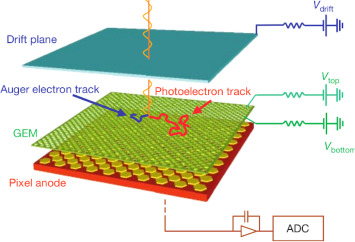
\includegraphics[scale=.85]{figures/gpd.jpg}
\caption{Design of the GPD. An incoming X-ray photon interacts with a gas molecule to produce a photoelectron between the entrance window and the gas electron multiplier (GEM). Secondary charges created along the photoelectron's path are multiplied by the GEM and read out at the anode plane. This forms a 2D photoelectron track image on hexagonal pixel grid; fig.~\ref{fig:tracks} gives some examples. Figure from \citet{baldini_design_2021}.}
\label{fig:gpd}       % Give a unique label
\end{figure}

\begin{figure}[t]
\centering
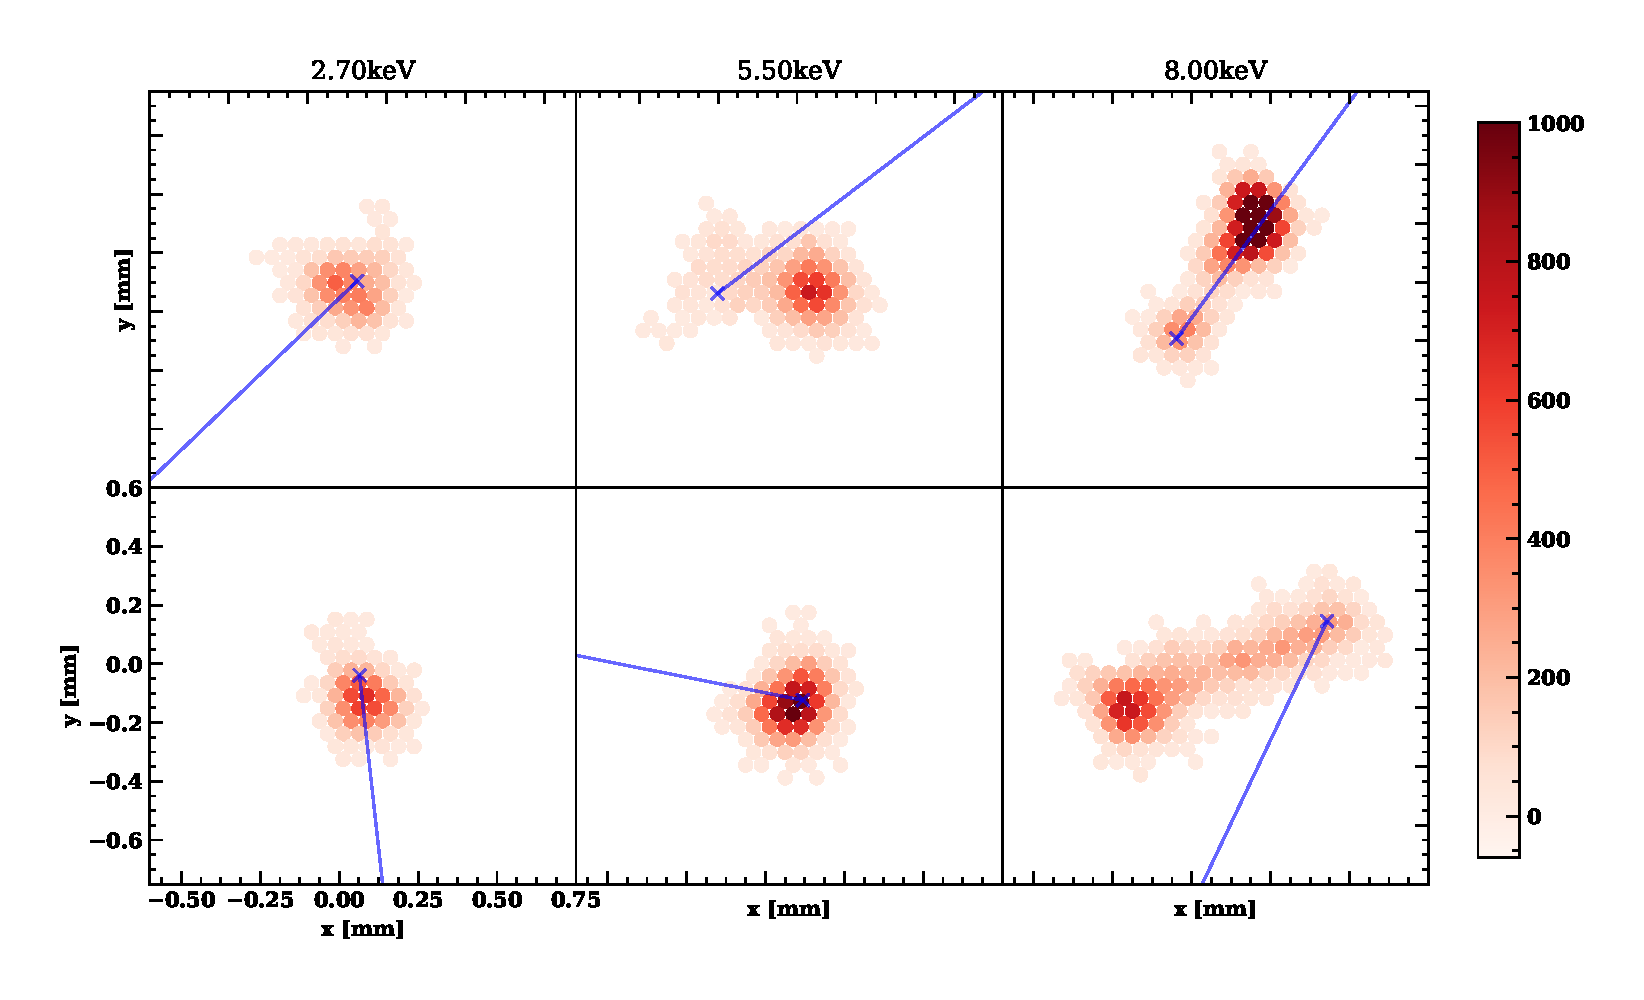
\includegraphics[scale=.5]{figures/fig1.pdf}
\caption{A selection of measured photoelectron track events from IXPE GPDs. Pixel color density represents charge deposited, blue crosses show photon x-y absorption point and blue lines the initial photoelectron direction. Pixels are thresholded at 10 counts. Track morphologies vary widely and depend strongly on energy.}
\label{fig:tracks}       % Give a unique label
\end{figure}

In the $1-15$ keV range, the cross-section for photoelectron emission is proportional to cos$^2(\theta - \theta_0)$, where $\theta_0$ is the normal incidence X-ray's electric vector position angle (EVPA) and $\theta$ the azimuthal emission direction of the photoelectron; see the previous chapter. 
Specifically, the emission angles $\theta$ follow the distribution 
\begin{equation}
    \theta \sim \frac{1}{2\pi} \big(1 + p_0\cos[2(\theta - \theta_0)] \big).
    \label{eqn:prob}
\end{equation}
By measuring a large number of individual photoelectron emission angles $\{\hat{\theta}_i\}_{i=1}^N$, one can recover the above distribution to extract the source polarization parameters: polarization fraction ($0 \leq p_0 \leq 1$) and EVPA ($-\pi/2 \leq \theta_0 < \pi/2$). In practice, the recovery of photoelectron emission angles from track images is imperfect. Track images are noisy due to Coulomb scattering and diffusion, and, especially for low energies, are often barely resolved. For example, in fig.~\ref{fig:mu} the distribution of recovered emission angles using IXPE's classical track reconstruction is significantly blurred compared to the true distribution.

The best classical track reconstruction method for GPDs is a moment analysis described by \citet{bellazzini_novel_2003} and in the previous chapter. Impressive accuracies for the emission angle and photon absorption point are achieved from a simple weighted combination of track moments. Photon energy estimates are proportional to the total collected GPD charge for a track. The track ellipticity is quantified to provide a rough proxy for track reconstruction quality. High ellipticity tracks typically have more accurate angle estimates. However, simple moments cannot capture all image information, especially for long high energy tracks, and so a more sophisticated image analysis scheme can lead to improved track emission angle, absorption point, and energy recovery.

Once the emission angles have been reconstructed, $\{\hat{\theta}_i\}_{i=1}^N$,
classical polarization estimation uses a maximum likelihood estimator (MLE) or direct curve fit to calculate $(\hat{p}_0, \hat{\theta}_0)$. This assumes individual tracks contribute equally to the final polarization estimate. In fact, photoelectron tracks are very morphologically diverse, even for the same photon energy (cf.~fig.~\ref{fig:tracks}), and so emission angle estimates are highly heteroskedastic: some emission angles are much better estimated than others. 
%they are mostly morphologically diverse because of the detector Z axis.
This is especially true for tracks of different photon energies, important in the case of broadband polarization estimates. Assuming an equal contribution from all estimated emission angles results in sub-optimal polarization recovery. 
To ameliorate this, IXPE's standard analysis performs an event cut removing tracks in the bottom $20\%$ of estimated ellipticities; this does provide a marginal improvement in the recovered polarization signal. However, a detailed analysis with proper estimation of emission angle uncertainties and their inclusion in the likelihood function can substantially improve the signal-to-noise ratio of recovered polarization. 


% A NN photoelectron track analysis has been recently described \citep{kitaguchi_convolutional_2019} for the detector geometry that was intended for the PRAXyS X-ray polarimetry mission \citep{tamagawa_x-ray_2017}. Using a convolutional neural network (CNN), they show significant improvements in electron angle and polarization recovery over a standard moment analysis for a square pixel grid polarimeter. While an excellent start, this analysis showed unexplained biases for unpolarized sources, used event cuts rather than weights and provide only a binned polarization analysis. 

\begin{figure}[t]
\centering
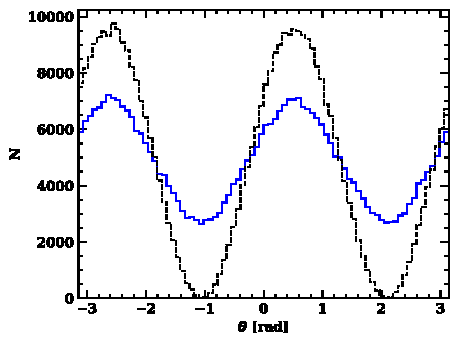
\includegraphics[scale=1]{figures/mod_example.pdf}
\caption{Photoelectron angles for a $100\%$ polarized ($p_0 = 1$) 6.4keV simulated line source. Black gives the true photoelectron angles, blue gives the recovered photoelectron angles for the standard moment analysis.}
\label{fig:mu}       % Give a unique label
\end{figure}

Measuring the X-ray polarization of a source using an imaging X-ray polarimeter is, from a data analysis perspective, a two step process. 
\begin{enumerate}
    \item \textit{Track reconstruction}. The telescope is pointed at the source and collects photoelectron track images, see fig.~\ref{fig:tracks}. Individual track images are processed to extract all of the relevant features: emission angles, absorption points and photon energies. \\
    
    \item \textit{Polarization estimation}. The extracted emission angles from many individual photoelectron tracks are combined to estimate the source polarization parameters.
\end{enumerate}
For spatially extended, time-varying or spectrally varying sources, the extracted emission angles could be grouped based on absorption points, arrival time or photon energy, i.e. in spatial, time and/or energy bins. Polarization estimation from these grouped emission angles follows the same procedure.

This chapter describes classical approaches for both steps, a prerequisite for the neural network approach. In classical polarization analysis the two steps are entirely disconnected. \S\ref{chap:sbi} will show how these two steps can be more closely connected using neural network uncertainty estimates.

\subsubsection{Track reconstruction}
\label{sec:trckrec}
Photoelectron track images contain all the extractable information in imaging X-ray polarimeters. More specifically, the various sensitivities of an imaging X-ray polarimeter can be attributed to a few photoelectron track features that can be extracted from individual track images:
\begin{itemize}
    \item \textit{Polarization sensitivity:} photoelectron emission angle $\theta$, \S\ref{sec:emit}.
    \item \textit{Spatial sensitivity:} photon absorption point $(x,y)$, \S\ref{sec:absp}.
    \item \textit{Spectral sensitivity:} photon energy $E$, \S\ref{sec:E}.
\end{itemize}
Tracks are imaged by charge deposition onto an array of pixels. For example, IXPE's GPD pixel array is a $\sim$ 15mm x 15mm square tiled with hexagonal pixels on a $50\mu$m pitch \citep{baldini_design_2021}; see fig.~\ref{fig:pix}. The charge deposited in each pixel is measured in integer counts, typically ranging from 0 to 1000+, fig.~\ref{fig:tracks}. Track images are identified on the pixel array by clustering analysis and the region of interest is cropped. Each track image comes as a list of $(x,y,c)$ tuples: the pixel coordinates $x,y$ and charge deposited $c$. 

There are a number of instrument specific settings that affect track morphology. For example, a pixelwise charge threshold is usually applied to individual track images to reduce small noisy pixel clusters. The GPD gas pressure and composition can also be varied; lower pressure allows for longer tracks that are easier to reconstruct but reduces the detector quantum efficiency. The methods presented in this chapter generalize to all imaging polarimeter settings, details on optimizing specific settings can be found in chapters XY. The examples shown here assume IXPE-specific GPD settings.

\begin{figure}[t]
\centering
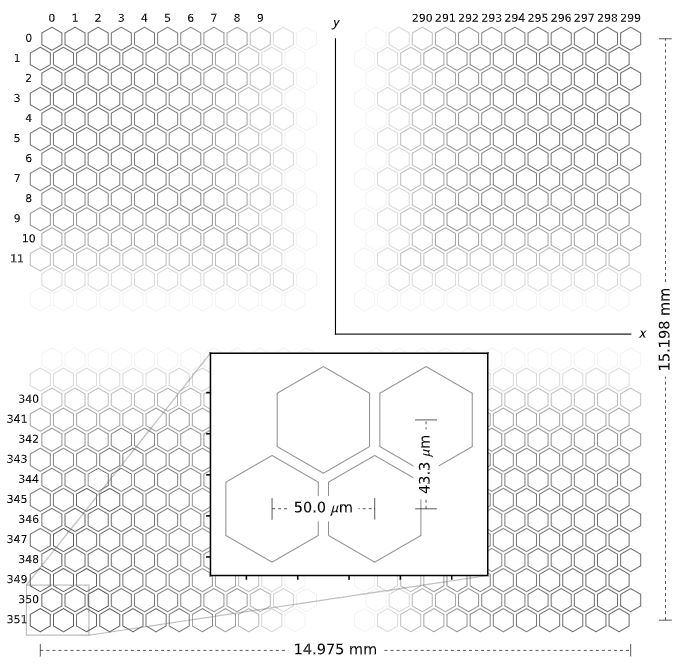
\includegraphics[scale=1]{ASIC.JPG}
\caption{Layout of IXPE GPD readout pixel array. There are approximately 90000 pixels. More pixels allow for better track reconstruction. Figure from \citet{bellazzini_novel_2003}.}
\label{fig:pix}       % Give a unique label
\end{figure}

\subsubsection{Emission angle reconstruction}
\label{sec:emit}
Source polarization is encoded in the photoelectron emission angles $\theta$. These are the image plane projected initial directions of the photoelectron at the interaction point. Track images capture the entire track of the photoelectron in the image plane, so in principle it should be possible to recover the initial direction.
In practice, track images are relatively noisy representations of the photoelectron path. Charge diffusion means the further away from the pixel array a photoelectron is emitted, the less well defined its track image will be.

Track images are typically asymmetric and follow a similar pattern: the photoelectron starts at the absorption point and moves along its initial direction. Sometimes an Auger electron is also released at the absorption point. As the photoelectron moves away from the absorption point, it is Coulomb scattered away from the initial direction. As the photoelectron slows down, it ionizes more gas molecules, depositing more charge in the pixel array and culminates in a final Bragg peak. Low energy photoelectrons travel less far from the absorption point and leave nearly circularly symmetric track images. %(figure of a single track with details added?)

The scattering of the photoelectron from its initial direction and short, symmetric photoelectron tracks make emission angle reconstruction challenging. The moment analysis described in \citet{bellazzini_novel_2003} uses the known structure of photoelectron tracks to improve their emission angle estimates. They initially calculate the principal axis of the track image by maximizing the second charge moment about the track barycenter. This provides a simple initial estimate of the emission angle, but is skewed by the Bragg peak -- the dense final part of the track that is usually not correlated to the initial direction because of Coulomb scattering. To correct for the Bragg peak bias, the location of the Bragg peak is calculated by observing the sign of the third charge moment about the track barycenter. This identifies which side of the track contains the Bragg peak. The absorption point is estimated as being a multiple of the second moment away from the track barycenter along the principal axis, away from the Bragg peak. Finally, the emission angle is calculated by using the second moment about the absorption point, using only pixels in the initial half of the track (those not on the Bragg peak side). See the previous chapter for more details on the moment analysis.

% On top of the blurry track images, the photoelectron path itself can be misleading. The photoelectron is likely to be scattered off its original direction the farther it travels from the absorption point. Photoelectrons that travel significantly into the image plane or low energy photoelectrons that barely move from the absorption point can leave highly symmetric tracks with unclear initial directions. Auger electrons can be emitted in addition to the photoelectron, potentially confusing the initial photoelecton direction.
% If the track images were time resolved it would be much easier to estimate the emission angle. 

\subsubsection{Absorption point reconstruction}
\label{sec:absp}
Photon absorption points $(x,y)$ on the image plane along with the known point spread function (PSF) of the telescope optics allow for the spatial resolution of extended sources. Better absorption estimates yield better spatial resolution. A simple estimator for the absorption point of an individual photon from its track image is the track barycenter, but this can be strongly biased by the photoelectron Bragg peak \S\ref{sec:emit}. In moment analysis \citep{bellazzini_novel_2003}, the absorption point is estimated jointly with the emission angle by identifying and excluding the Bragg peak.
For low energy symmetric tracks where it is impossible to separate the Bragg peak, the track barycenter is used as the standard absorption point estimator.
%(Plot of full detector grid with lots of tracks). 

% Determine precise absorption point of photon on detector grid. For example, IXPE's GPD hexagonal pixel array is a 7mm x 7mm square, where each pixel is 50$\mu$m
% PSF of the telescope optics will dictate distribution of tracks on the pixel array.
% (Plot of full detector grid with lots of tracks). 
% Track barycenters provide better estimate at low energies.

\subsubsection{Energy reconstruction}
\label{sec:E}
An X-ray photon's energy is proportional to the average charge deposited in the detector. Since the charge deposited is subject to statistical fluctuations, the energy resolution is limited and this limit depends on the effective detector Fano factor. Classical polarimetry uses a simple linear model calibrated on real detector track images to reconstruct the photon energy. Thus, the total track charge is assumed proportional to the photon energy. This method approaches but does not meet the theoretical best energy resolution.
% Simple linear model, should be easy peasy.
% 1-10keV, low effective area outside of this for IXPE.

\begin{figure}[t]
\centering
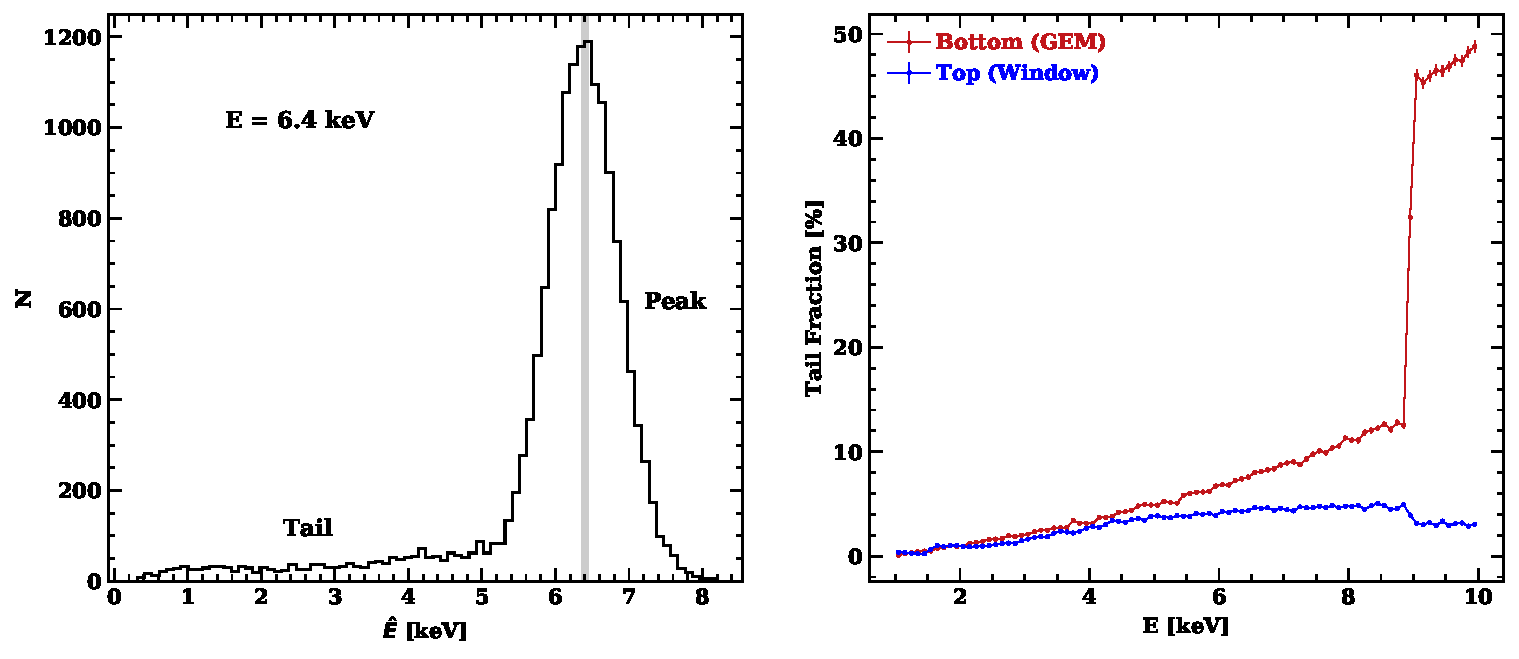
\includegraphics[width=1\textwidth]{figures/fig3.pdf}
\caption{\textit{Left:} Recovered energy histogram for a 6.4keV line source. A simple linear function of total charge deposited is used here for recovered energy, as in the standard moment analysis. The long low energy tail is produced by events converting in the window or GEM. \textit{Right:} Fraction of events that are `tails' as a function of energy. Red and blue traces show the Be window and GEM conversion respectively. The jump in GEM conversions at 8.9\,keV Cu edge is prominent.}
\label{fig:tails}       % Give a unique label
\end{figure}

\subsubsection{Events converting outside of the gas volume}
\label{sec:tail}
So far, the track images considered are formed when photons interact with the detector gas. However, incoming X-ray photons can also convert in detector components just outside of the main gas volume, with electrons penetrating the gas triggering the GPD and producing photoelecton tracks. For IXPE's GPDs, these external interactions occur in the thin beryllium entrance window at the top of the GPD and in the gas electron multiplier copper material at the bottom, fig.~\ref{fig:gpd}. The track images formed by these external interactions have different morphological properties compared to those in the detector gas. Notably, they have less total charge deposited for the same photon energy, because some of the photoelectron energy can be lost in the solid window or GEM material. In addition they tend to have a denser `core' since the photoelectrons surviving to the gas volume tend to have trajectories with a large vertical component. The left panel of fig.~\ref{fig:tails} shows the linearly reconstructed energy (\S\ref{sec:E}) for a 6.4keV line source. External events form a low energy tail on the predicted energy histogram -- external events are described here tail events, producing tail tracks, while events converting in the detector gas are called peak events. The right panel gives the population fraction of tail events as a function of photon energy. Tail tracks are mostly subdominant, but with a linearly increasing fraction as photon energy increases. At energies above 8.9 keV, the Copper K absorption edge causes a large increase in tail events in the GEM, increasing the tail track fraction.

\begin{figure}[t]
\centering
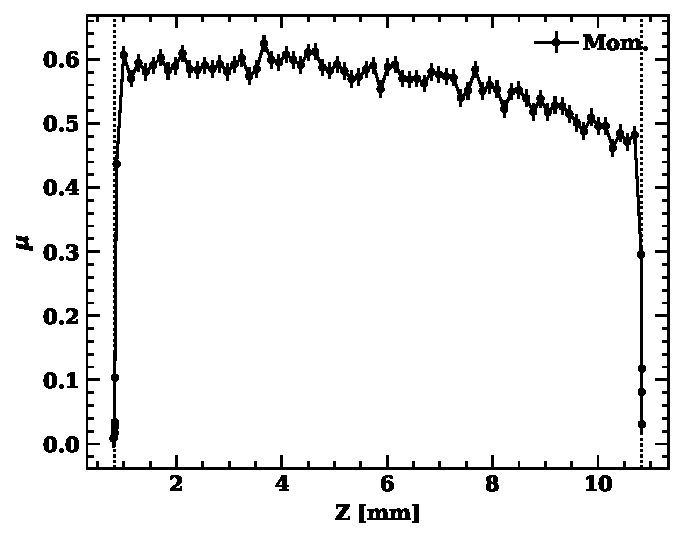
\includegraphics[scale=.75]{figures/z_mu.pdf}
\caption{Polarization sensitivity, measured by the modulation factor $\mu$ (\S\ref{sec:polest}), as a function of absorption point height in IXPE's GPD. Dotted lines denote the edges of the GPD, the top at z=10.83mm is the Beryllium window, and the bottom at z=0.83mm is the Cu-coated GEM.}
\label{fig:z}       % Give a unique label
\end{figure}

Tail tracks also have significantly reduced polarization signal compared to peak tracks. The emitted photoelectron is scattered more strongly in the dense GEM and window materials than in the detector gas; as a result, the initial photoelectron direction is often irrecoverable. Fig.~\ref{fig:z} gives the simulated polarization sensitivity as a function of vertical direction along IXPE's GPD, using the moment analysis to estimate photoelectron emission angles. There is a clear drop in sensitivity at both vertical edges of the detector where tail tracks dominate the absorption. Additionally, this figure serves to illustrate the decrease in polarization sensitivity with increasing vertical distance from the pixel array. This is due to charge diffusion in the detector gas blurring tracks before they reach the pixel read-out array (\S\ref{sec:emit}).

If included, tail tracks can cause problems during polarization estimation. Not only do tail tracks degrade the detector polarization sensitivity, the energy-dependent tail fraction can make it difficult to properly calibrate the polarization sensitivity and degrade the energy resolution for continuous spectra. In classical imaging polarimetry, tail tracks are cut from the line source calibration by excluding the low energy tail from the recovered energy histogram, fig.~\ref{fig:tails}. For real, continuous sources this is not possible, so tail tracks remain an important problem for classical polarimetry approaches. \S\ref{sec:removetail} will describe how a NN analysis can identify tail tracks based on their morphological differences and decrease their contamination of the polarization signal.

\subsection{Polarization estimation}
\label{sec:polest}
Polarization estimation can begin once all relevant track features have been recovered. The basic problem is to estimate source polarization parameters $(p_0,\theta_0)$ and their uncertainties from a set of reconstructed emission angles $\{\hat{\theta}_i\}_{i=1}^N$.  As described in the introduction, true emission angles $\theta$ exhibit a sinusoidal modulation with period $\pi$ that depends on the source polarization
\begin{equation} \label{eqn:likelihood}
    p(\theta|p_0,\theta_0) = \frac{1}{2\pi}\big(1 + p_0{\rm cos}\big[2(\theta - \theta_0)\big]\big),
\end{equation}
where $0 \leq p_0 \leq 1$, $-\pi/2 \leq \theta_0 < \pi/2$ and $-\pi \leq \theta < \pi$. Reconstructed emission angles $\hat{\theta}$ are imperfectly recovered, so these follow an adjusted distribution
\begin{equation} \label{eqn:likelihoodmu}
    p(\hat{\theta}|p_0,\theta_0) = \frac{1}{2\pi}\big(1 + p_0\mu{\rm cos}\big[2(\hat{\theta} - \theta_0)\big]\big).
\end{equation}
The modulation factor $0 \leq \mu \leq 1$ is a measure of the detector polarization sensitivity: how well the emission angles are recovered. A higher modulation factor means better polarization sensitivity and $\mu = 1$ means perfect emission angle reconstruction, $\theta = \hat{\theta}$. The modulation factor is the recovered polarization fraction $\hat{p}_0$ for a 100\% polarized source, $p_0 = 1$. Fig.~\ref{fig:mu} gives an example for a $p_0 = 1$ source, the moment analysis recovered emission angles follow the blue $\mu < 1$ distribution while the true emission angles have $\mu = 1$. The modulation factor is a function of photon energy, higher energy tracks have higher modulation factor because they have longer tracks, thus better emission angle estimates. Track reconstruction algorithms and detector hardware both affect the instrument modulation factor. The modulation factor can be considered an average of the reconstruction quality of all tracks for a particular source energy spectrum.  In \S\ref{chap:sbi} we will revisit the modulation factor from first principles; for now it can be treated as a known constant for a given source energy spectrum, determined by instrument calibration.

\subsubsection{Stokes parameters}
It is usually simpler to estimate the normalized linear Stokes parameters $(\mathcal{Q}, \mathcal{U})$ instead of the polarization fraction and EVPA $(p_0, \theta_0)$. These are an alternative representation of the source linear polarization. Disregarding circular polarization, the Stokes parameters are defined as
\begin{equation}
    Q = Ip_0\cos2\theta_0,
    \label{eqn:q1}
\end{equation}
\begin{equation}
    U = Ip_0\sin2\theta_0,
    \label{eqn:u1}
\end{equation}
where $I$ is the source intensity, and the normalized Stokes parameters are
\begin{equation}
    \mathcal{Q} = p_0\cos2\theta_0,
    \label{eqn:qq1}
\end{equation}
\begin{equation}
    \mathcal{U} = p_0\sin2\theta_0,
    \label{eqn:uu1}
\end{equation}
$-1 \leq \mathcal{Q} \leq 1$, $-1 \leq \mathcal{U} \leq 1$, from which the polarization fraction and EVPA can be derived:
\begin{equation}
    p_0 = \sqrt{\mathcal{Q}^2 + \mathcal{U}^2},
    \label{eqn:p}
\end{equation}
\begin{equation}
    \theta_0 = \frac{1}{2}\arctan\frac{\mathcal{U}}{\mathcal{Q}}.
    \label{eqn:th}
\end{equation}
Using Stokes parameters, the probability density eq.\ref{eqn:likelihoodmu} can be rewritten
\begin{equation}
    p(\hat{\theta}|\mathcal{Q},\mathcal{U}) =  \frac{1}{2\pi} \big(1 + \mathcal{Q}\mu\cos2\hat{\theta} + \mathcal{U}\mu\sin2\hat{\theta} \big).
    \label{eqn:prob_stokes}
\end{equation}
This is a more convenient form because the probability density is linear in the Stokes parameters, unlike for $(p_0, \theta_0)$. Some researchers even prefer to work solely with Stokes parameters. Since likelihoods are invariant to reparameterization, estimating the Stokes parameters and converting back to $(p_0, \theta_0)$ is equivalent to estimating $(p_0, \theta_0)$ directly, although some care must be taken in propagating the uncertainties.

\subsubsection{Methods}
With the modulation factor known, $(p_0, \theta_0)$ and/or $(\mathcal{Q}, \mathcal{U})$ can be recovered from the emission angles $\{\hat{\theta}_i\}_{i=1}^N$ in a number of ways. The simplest method is a binned curve fit, i.e. directly fitting the probability density eq.\ref{eqn:prob_stokes} to the histogram of emission angles $\{\hat{\theta}_i\}_{i=1}^N$, fig.\ref{fig:mu}. Since the Stokes parameters are linear in the probability density eq.\ref{eqn:prob_stokes} they can be fit using binned least squares. The resulting estimates $(\hat{\mathcal{Q}},\hat{\mathcal{U}})$ are unbiased and equivalent to the maximum likelihood estimator (MLE), so long as the bin widths are small enough and each bin contains enough events such that Poisson statistics can be well approximated by Gaussian. This is not always the case, so directly applying the MLE is often a better approach. 

The MLE is the estimator $(\hat{\mathcal{Q}},\hat{\mathcal{U}})$ that maximizes the likelihood function:
\begin{equation}
    L(\{\hat{\theta}_i\}_{i=1}^N|\mathcal{Q},\mathcal{U}) =  \prod_{i=1}^N\frac{1}{2\pi} \big(1 + \mathcal{Q}\mu\cos2\hat{\theta}_i + \mathcal{U}\mu\sin2\hat{\theta}_i \big).
    \label{eqn:likelihood_stoks}
\end{equation}
Here $L$ is a function of $(\mathcal{Q},\mathcal{U})$ and the observations $\{\hat{\theta}_i\}_{i=1}^N$ are fixed. Computationally, it is easier to minimize the negative log-likelihood function
\begin{equation}
    -\log L =  N\log 2\pi - \sum_{i=1}^N \log \big(1 + \mathcal{Q}\mu\cos2\hat{\theta}_i + \mathcal{U}\mu\sin2\hat{\theta}_i \big).
    \label{eqn:loglikelihood_stoks}
\end{equation}
This expression must be minimized numerically to find $(\hat{\mathcal{Q}},\hat{\mathcal{U}})$. Confidence intervals are calculated by numerically integrating the negative log likelihood function in the vicinity of the final estimator. Stokes parameter estimators and their errors can be simply transformed into $(\hat{p}_0,\hat{\theta}_0)$ if desired.

It is often inconvenient to evaluate the MLE and its errors numerically. An analytical solution for the MLE exists if $|\mathcal{Q}\mu| << 1, |\mathcal{U}\mu| << 1$. In practical X-ray polarimetry this limit is nearly always satisfied; polarimeters typically do not achieve much better than $\mu \lesssim 0.5$ averaged over a continuous spectrum and real astrophysical sources generally have low polarization $p_0 \lesssim 0.3$. By applying the Taylor expansion $\log(1+x) \approx x - x^2/2$  to the negative log-likelihood eq.~\ref{eqn:loglikelihood_stoks} and minimizing the resulting quadratic form one finds

\begin{equation}
    \hat{\mathcal{Q}} = \frac{1}{\mu}\frac{(\sum^N_{i=1}\cos2\hat{\theta}_i -  \sum^N_{i=1}\cos2\hat{\theta}_i\sin2\hat{\theta}_i) \sum^N_{i=1}\sin^22\hat{\theta}_i}
    {\sum^N_{i=1}\cos^22\hat{\theta}_i \sum^N_{i=1}\sin^22\hat{\theta}_i - (\sum^N_{i=1}\cos2\hat{\theta}_i\sin2\hat{\theta}_i)^2},
    \label{eqn:qquadform}
\end{equation}

\begin{equation}
    \hat{\mathcal{U}} =  \frac{1}{\mu}\frac{(\sum^N_{i=1}\sin2\hat{\theta}_i -  \sum^N_{i=1}\cos2\hat{\theta}_i\sin2\hat{\theta}_i) \sum^N_{i=1}\cos^22\hat{\theta}_i}
    {\sum^N_{i=1}\cos^22\hat{\theta}_i \sum^N_{i=1}\sin^22\hat{\theta}_i - (\sum^N_{i=1}\cos2\hat{\theta}_i\sin2\hat{\theta}_i)^2}.
    \label{eqn:uquadform}
\end{equation}
Notice that $\mathbb{E}[\sum_{i=1}^N\cos2\hat{\theta}_i\sin2\hat{\theta}_i] = 0$, $\mathbb{E}[\sum_{i=1}^N\cos^22\hat{\theta}_i] = N/2$ and $\mathbb{E}[\sum_{i=1}^N\sin^22\hat{\theta}_i] = N/2$. For the relatively large $N$ in X-ray polarimetry, these terms are effectively constants, so the expressions reduce to
\begin{equation}
    \hat{\mathcal{Q}} = \frac{2}{N\mu} \sum^N_{i=1}\cos2\hat{\theta}_i,
    \label{eqn:qest}
\end{equation}
\begin{equation}
    \hat{\mathcal{U}} = \frac{2}{N\mu} \sum^N_{i=1}\sin2\hat{\theta}_i.
    \label{eqn:uest}
\end{equation}
Because these are unbiased and MLE, they are the minimum variance unbiased estimators for $(\mathcal{Q}, \mathcal{U})$. In other words, so long as $|\mathcal{Q}\mu| \lesssim < 1, |\mathcal{U}\mu| \lesssim < 1$ and $N \gtrsim 1000$, these are the best possible estimators for $(\mathcal{Q}, \mathcal{U})$.

\begin{figure}[t]
\centering
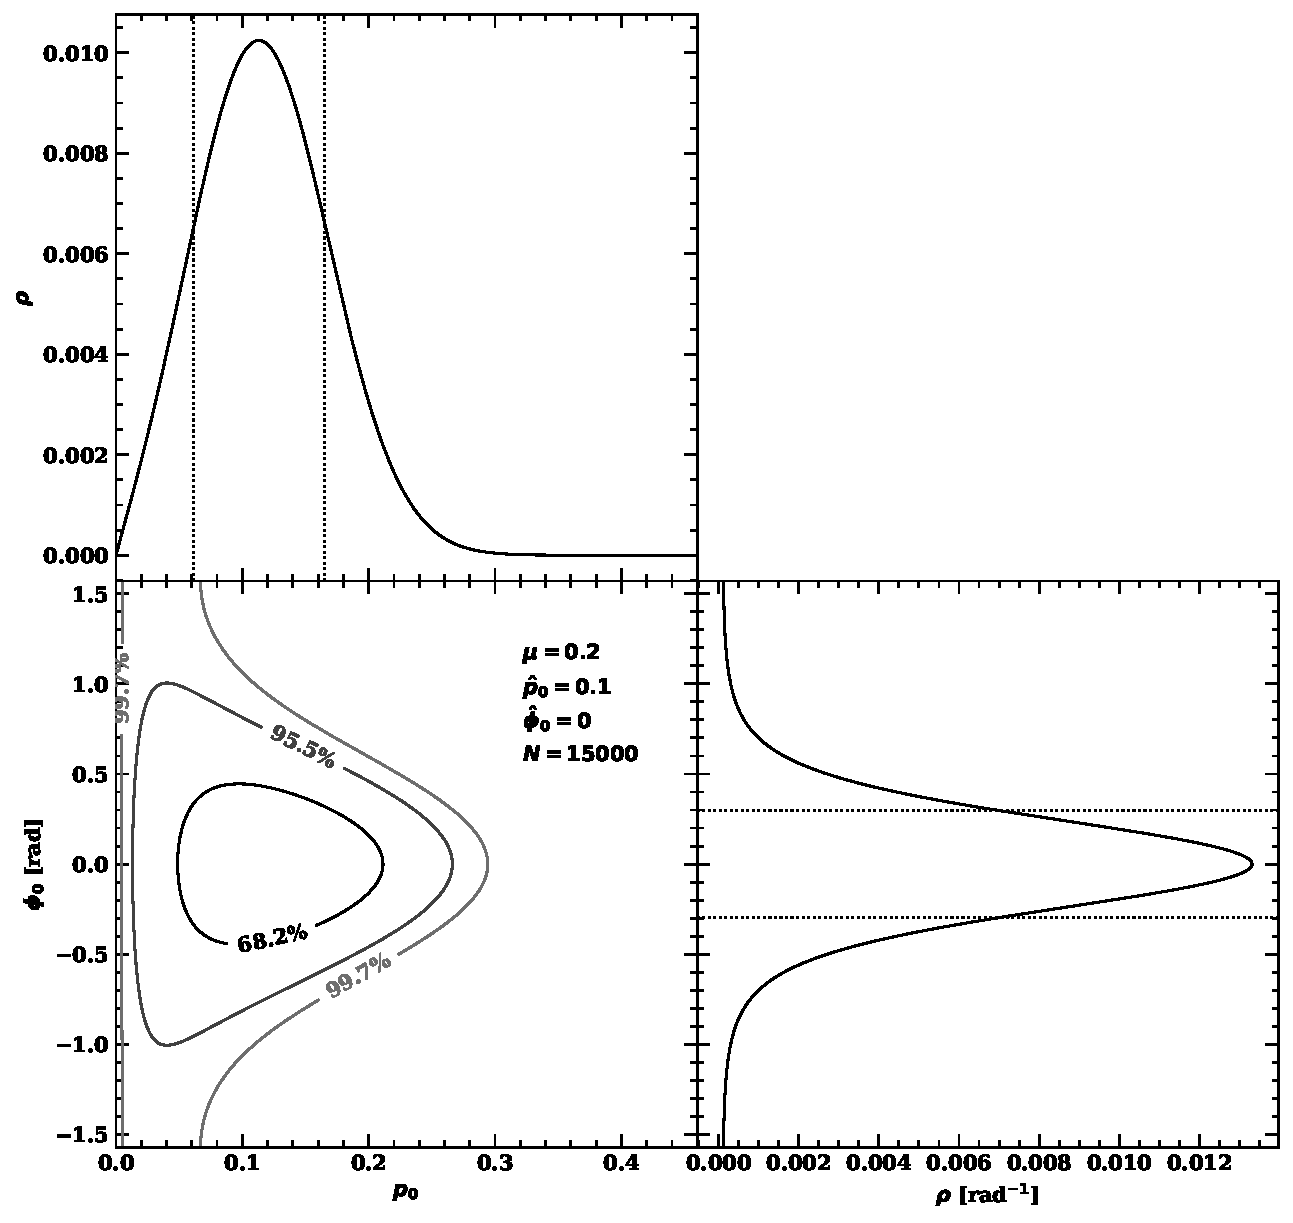
\includegraphics[scale=.5]{figures/contours.pdf}
\caption{Confidence intervals from full posterior distribution (eq.\ref{eqn:posterior}) over polarization parameters $(p_0, \phi_0)$ given estimates $(\hat{p}_0, \hat{\phi}_0)$ using $N$ events and instrument modulation factor $\mu$. 
Confidence intervals for $68.2\%$,$95.5\%$ and $99.7\%$ (1$\sigma$, $2\sigma$, $3\sigma$) are displayed.
The full marginal posterior distributions are plotted on the wings with $68.2\%$ (1$\sigma$) confidence intervals drawn. }
\label{fig:post}       % Give a unique label
\end{figure}


\citet{kislat_analyzing_2015} derive the full analytical posterior distribution for both $(\mathcal{Q},\mathcal{U})$ and $(p_0,\theta_0)$ given the estimators eqs.\ref{eqn:qest},\ref{eqn:uest}. They find the $(\mathcal{Q},\mathcal{U})$ posterior follows a bivariate normal distribution while the $(p_0,\theta_0)$ posterior is
\begin{equation}
\begin{aligned}
    p(p_0,\theta_0 | \hat{p}_0,& \hat{\theta}_0) ={} \frac{\sqrt{N}\hat{p}_0 \mu^2}{2\pi\sigma} \times \\
    &\exp\Bigg[-\frac{\mu^2}{4\sigma^2}\Bigg\{ \hat{p}_0^2 + p_0^2 - 2\hat{p}_0 p_0\cos(2(\hat{\theta}_0 - \theta_0)) \\ & - \frac{\hat{p}_0^2p_0^2\mu^2}{2}\sin^2(2(\hat{\theta}_0 - \theta_0)) \Bigg\} \Bigg],
\end{aligned}
\label{eqn:posterior}
\end{equation}
where 
\begin{equation}
    \sigma = \sqrt{\frac{1}{N} \left( 1 - \frac{p_0^2\mu^2}{2}\right)}.
    \label{eqn:sig}
\end{equation}
The posterior assumes a uniform prior over $(p_0,\theta_0)$. With the posterior in hand, any desired confidence interval can be computed analytically or numerically. 
High $\mu$ and high $N$ reduce the width of the posterior so are both desirable to minimize the errors on recovered polarization parameters.
Note that the estimator $\hat{p}_0$ is not unbiased, its posterior is highly asymmetric for low $p_0$ since $p_0 \geq 0$. For $p_0 = 0$ some polarization fraction $\hat{p}_0 > 0$ will always be measured. The amount of polarization likely to be measured when $p_0 = 0$ depends on the width of the posterior, i.e. $N$ and $\mu$, and is often used as a measure of detector sensitivity or signal-to-noise ratio (SNR), \S\ref{sec:mdp}.
Fig.~\ref{fig:post} shows the posterior distribution for an example observation.


The recommended approach to polarization estimation is using eqs.~\ref{eqn:qest}, \ref{eqn:uest} for point estimates and the derived posterior eq.~\ref{eqn:posterior} for confidence intervals. This approach is expedient and optimal given the instrumental constraints of imaging X-ray polarimetry. In \S\ref{chap:sbi} we extend eqs.~\ref{eqn:qest} -- \ref{eqn:posterior} to include neural network uncertainty estimates on predicted emission angles $\hat{\theta}$.


% list
% curve fitting
% maximum likelihood estimation
% Stokes analysis
% p0 estimate always biased, check the paper about p0 dsitribution.
% MDP99
% Plot of convergence of different $p_0, \theta_0$ estimation algorithms.




\subsubsection{Minimum detectable polarization (MDP)}
\label{sec:mdp}

The standard figure-of-merit used in X-ray polarimetry to compare instrument sensitivity is minimum detectable polarization (MDP) \citep{weisskopf_understanding_2010}. MDP$_{99}$ is the polarization fraction that has a 1\% probability of being exceeded by chance for an unpolarized ($p_0 = 0$) source. This can be found by integrating the posterior distribution eq.\ref{eqn:posterior}:
\begin{equation}
    \int_0^{\rm MDP_{99}} \int_{-\pi/2}^{\pi/2} p(p_0, \theta_0 | \hat{p}_0, \hat{\theta_0})d\theta_0 dp_0 = 0.99,
\end{equation}
\begin{equation}
    {\rm MDP}_{99} = \frac{4.29}{\mu\sqrt{N}}.
\end{equation}
On fig.~\ref{fig:post}, the MDP$_{99}$ would be the one sided $99\%$ confidence interval for the $p_0$ marginal distribution (top panel).
%Was a bit inconsistent with notation here

The MDP$_{99}$ depends only on the modulation factor (signal) and the Poisson counting noise $1/\sqrt{N}$; it is effectively an inverse of the SNR. Polarimeters with lower MDP$_{99}$ can expose for shorter times and get the same confidence on their polarization measurements. Track reconstruction and polarization estimation approaches that increase the modulation factor for a fixed number of tracks $N$ will decrease the MDP$_{99}$. Sections \ref{chap:nn} and \ref{chap:sbi} will describe how a neural network approach can improve both track reconstruction and polarization estimation to minimize the MDP$_{99}$.

\subsection{Neural Networks for Machine Learning}

Deep neural networks (DNNs) are a type of supervised machine learning algorithm. Machine learning algorithms learn from data, as opposed to a fixed algorithm programmed by human beings. Supervised machine learning algorithms learn from labelled data: known input-output pairs $\{x_i,y_i\}^N_{i=1}$. An example from X-ray polarimetry would be track image (input), emission angle (output). Supervised machine learning algorithms can be used to solve a variety of tasks. Most tasks belong to one of two groups: regression or classification. In regression the algorithm is trained to predict a continuous numerical value given an input. In classification, the algorithm predicts the probability an input belongs to a particular class from a preselected group of finite classes. In the case of track reconstruction, we are interested mainly in regression.

In essence, DNNs approximate the unknown function $f^{\star}$ that maps problem inputs to outputs $y = f^{\star}(x)$. DNNs are organized as a forward network of function layers each with their own learnable parameters or weights $w$, e.g. $f(x) = f_3(f_2(f_1(x;w_1);w_2);w_3)$. The initial function layer $f_1$ is known as the input layer, the final layer $f_3$ is the output layer, and all layers in between are the hidden layers. Using many hidden layers tends to improve the predictive capacity of the DNN, whence the term 'deep learning'. During training, the DNN $f(x)$ is iteratively directed towards $f^{\star}(x)$.

\begin{figure}[t]
\centering
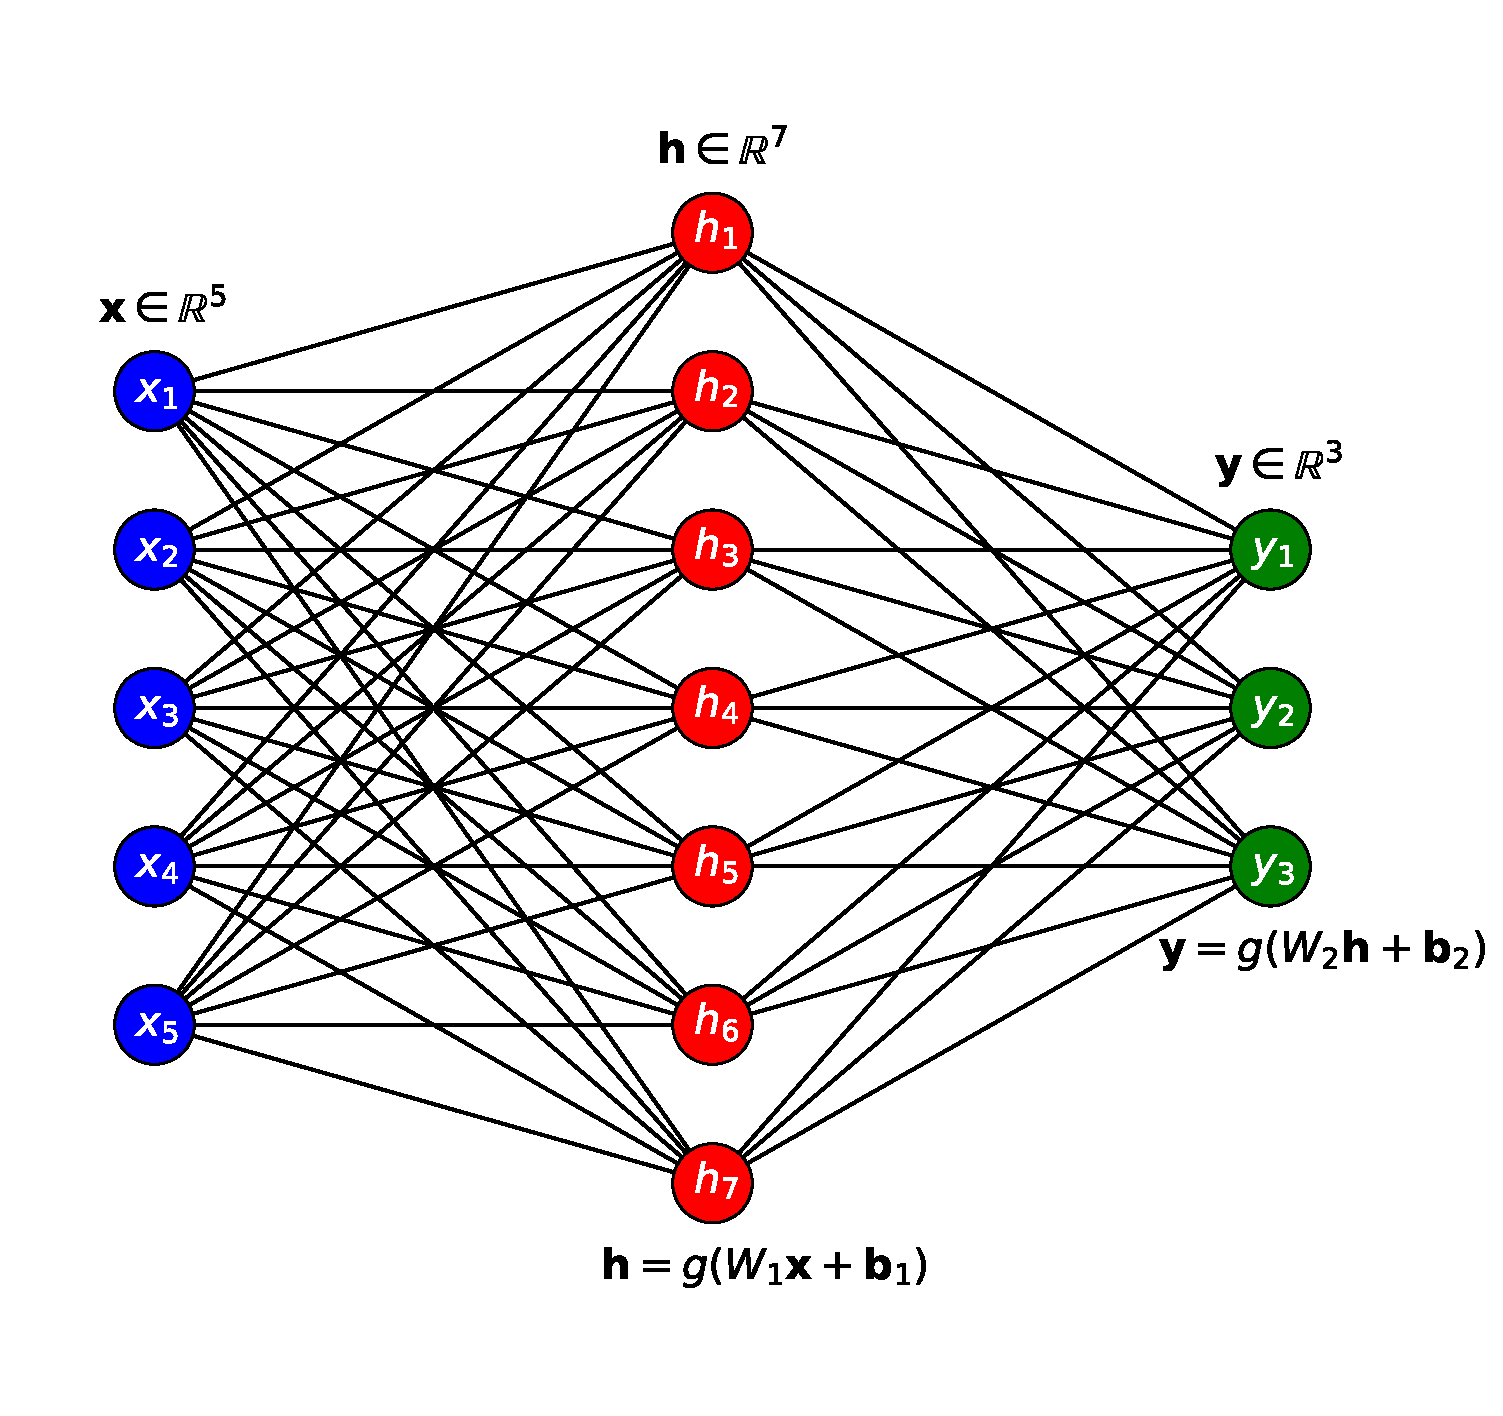
\includegraphics[scale=.35]{figures/network.pdf}
\caption{Feed-forward neural network with one hidden layer. The neural network takes vector $\mathbf{x}$ as input and produces vector $y$ as output.}
\label{fig:net}       % Give a unique label
\end{figure}

If the layer functions $f_1, f_2, f_3$ were linear then the DNN $y = f(x)$ would be a linear model $y = w^Tx$, equivalent to a simple least squares approach. DNNs use non-linear layer functions. This allows the DNN to learn non-linear relationships between the input features $y = w_2^Tf_1(x; w_1)$. Here $f_1(x;w_1)$ is a non-linear function with learnable parameters $w_1$.
In this way DNNs are able to learn what functions of the input features should be combined, unlike a linear model that linearly combines input features directly.
A simple example of a non-linear layer function used in DNNs is $f_1(x;w_1,b) = g(w_1^Tx + b)$ where $w_1$ is a matrix and $g$ is a non-linear function such as $\tanh$, the sigmoid function or a rectified linear unit (ReLU). DNNs using this kind of layer are universal function approximators in the asymptotic limit \citep{hornik_multilayer_1989}, so they should in principle well approximate any $f^{\star}(x)$. In practice, memory, training and data limitations make this difficult to achieve. Many DNNs use domain specific layer functions and architectures to reduce these limitations and converge to $f^{\star}(x)$ more quickly, see \S\ref{sec:CNN}. Figure \ref{fig:net} shows a schematic of a simple DNN.

\subsubsection{Training}
\label{sec:training}
As in supervised linear models like least squares regression, DNNs are trained to minimize a specific loss function over the observed data. In most tasks this normally means minimizing the negative log-likelihood, as in \S2.2. For regression tasks, if the output distribution family $p(y|x)$ is unknown, a Gaussian should usually be the default since it is the least informative choice. For a Gaussian likelihood, the negative log likelihood is 
\begin{equation}
    L(\{y_i,x_i\}_{i=1}^N\mid\mathbf{w}) \propto \sum^N_{i=1}\|y_i - \hat{y}(x_i|\mathbf{w})\|^2,
    \label{eqn:egloss}
\end{equation}
the mean squared error (MSE) of prediction for the dataset. The loss function $L(\mathbf{w})$ is minimized over the DNN weights $\mathbf{w}$. MSE is a common loss function for regression with DNNs.

For classification tasks, $p(y|x)$ is usually assumed to follow a Bernoulli (in binary, 2-class classification) or categorical distribution (in >2 class classification). In the Bernoulli case, the negative log-likelihood is
\begin{equation}
    L(\{y_i,x_i\}_{i=1}^N\mid\mathbf{w}) \propto \sum^N_{i=1} - y_i\log\big(\hat{y}(x_i|\mathbf{w})\big) - (1 - y_i)\log\big(1 - \hat{y}(x_i|\mathbf{w}) \big).    
    \label{eqn:eglossbin}
\end{equation}
In order to ensure $0 \leq \hat{y}_i \leq 1$, DNNs for classification usually end with a softmax layer \citep{bridle_training_1990}. These project DNN outputs onto the appropriate simplex, i.e., makes sure all predicted probabilities sum to one. For K output classes
\begin{equation}
    \label{eqn:softmax}
    {\rm Softmax}(\mathbf{x})_i = \frac{e^{x_i}}{\sum_{i=1}^K e^{x_i}}
\end{equation}

Since DNNs use non-linear functions, eq.~\ref{eqn:egloss} or \ref{eqn:eglossbin} cannot be minimized analytically. Non-linearity makes the loss function complex with multiple local minima and saddle points in a very high dimensional weight space $\{\mathbf{w}\}$. %non-convex
This challenging minimization problem is usually tackled with variations on the stochastic gradient descent (SGD) algorithm \citep{goodfellow_deep_2016}. At each iteration SGD approximates the gradient of the loss function using a subset of the training data
\begin{equation}
    g_i = \nabla_{\mathbf{w}} L(\mathbf{w}) \approx \sum_{i=1}^n \nabla_{\mathbf{w}}\|y_i - \hat{y}(x_i|\mathbf{w})\|^2, ~~n << N
\end{equation}
and takes a step in parameter ($\mathbf{w}$) space along the direction of the negative gradient
\begin{equation}
    \mathbf{w}_{i+1} = \mathbf{w}_{i} - \epsilon g_i.
\end{equation}
The process is repeated until suitable convergence. The weights are initialized randomly and the learning rate $\epsilon$ is a tuneable scalar for the specific application. The gradient for each individual $w_i$ can be calculated by using the chain rule through each layer of the DNN, in a process called backpropagation \citep{goodfellow_deep_2016}. In order for SGD to work, the DNN has to use a differentiable loss function and layer functions $f_1,f_2,f_3$. 
The whole dataset $N$ is not used to calculate the gradient because it is too slow and often too large to fit into memory. Furthermore, DNNs benefit from using small batches $n$ to approximate the gradient because the added stochasticity lets the minimization escape saddle points and local minima \citep{goodfellow_deep_2016}. Usually DNNs are trained on graphical processing units (GPUs), specialized computer hardware for fast and parallelizable linear algebra operations. 

\subsubsection{Validation and model selection}
\label{sec:val}
DNNs typically have on the order of millions, sometimes billions \citep{brown_language_2020}, of trainable weights $\mathbf{w}$. The number of weights is often higher than the number of training examples, making overfitting the labelled dataset likely. This is the central challenge of machine learning: the algorithm must perform well on new inputs, not just those in the training dataset. To ensure model generalization to unseen examples, part of the training data is set aside for validation. 
The trainable weights $\mathbf{w}$ are not trained on these examples.
DNNs come with a number of additional model parameters -- hyperparameters -- that can be adjusted to improve model generalization; examples include the learning rate $\epsilon$, the neural network architecture (type and number of layers) and any regularization. During training, the DNN is evaluated on the validation examples to tune the hyperparameters. This process is known as model selection. %More complex procedures for model selection can be used, such as k-fold cross-validation \citep{hastie_elements_2009}.  

Regularization is an important hyperparameter for improving model generalization. In exactly the same way as linear models can be regularized, for example in ridge regression, one can regularize a DNN by adding a penalty on the weights $\mathbf{w}$ to the loss function. A common example is L2 regularization:  
\begin{equation}
    L(\mathbf{w}) \propto \lambda\|\mathbf{w}\|^2 + \sum^N_{i=1}\|y_i - \hat{y}(x_i|\mathbf{w})\|^2.
    \label{eqn:regloss}
\end{equation}
The additional term restricts the model space by encouraging the weights $\mathbf{w}$ to be close to zero. The hyperparameter $\lambda$ can be tuned to maximize generalization on the validation examples. This type of regularization is equivalent to a Gaussian prior on the weights with mean zero. By restricting the model space, regularization helps prevent overfitting and improves generalization when $\lambda$ is appropriately tuned.

\subsubsection{Convolutional Neural Networks}
\label{sec:CNN}
Some DNNs have specialized layer functions that provide an inductive bias helpful for specific inputs. Convolutional neural networks (CNNs) \citep{lecun_convolutional_1998} were designed for processing inputs that have neighbouring position correlations, for example 2D images, where adjacent pixel values are often correlated, or 1D time series where adjacent time points are often correlated. CNNs use layer functions that apply a convolution to the input. The convolution kernel function is learned during training. This kind of layer function is invariant under translation of the input, an important prior for working with image data.
CNNs have revolutionized image processing and computer vision applications since winning the Imagenet benchmark competition in 2012 \citep{krizhevsky_imagenet_2012}.  
(Paragraph and plot of convolution here maybe)

Recently, a certain class of CNNs called residual networks (ResNets) have achieved state-of-the-the-art results in multiple image benchmark tasks \citep{he_deep_2015}. ResNets introduce 'skip' connections between certain layers that allow the CNN to ignore the layers in between. This alleviates many of the difficulties in training extremely deep neural networks.

\subsubsection{Multitask learning}
\label{sec:multi}
So far, only DNNs with single objectives and outputs have been considered. However, DNNs can be trained to solve multiple tasks at once, producing a vector of outputs. Solving multiple tasks at once often performs better than solving each task individually. This is partly because multiple tasks have a regularizing effect on each other, penalizing model complexity and overfitting on any single task leading to better overall model generalization \citep{zhang_survey_2021}. Moreover, since each task shares the same input representation, e.g., an image, the features learned for a single task can help the others train faster and better.

In a multitask learning setting, the loss function includes the terms for each individual task. For example, in regression with three tasks and an MSE loss for each
\begin{equation}
    L(\mathbf{w}) \propto \sum^N_{i=1}\|y^1_i - \hat{y}^1(x_i|\mathbf{w})\|^2 + \alpha\sum^N_{i=1}\|y^2_i - \hat{y}^2(x_i|\mathbf{w})\|^2 + \beta\sum^N_{i=1}\|y^3_i - \hat{y}^3(x_i|\mathbf{w})\|^2,
    \label{eqn:megloss}
\end{equation}
where the DNN outputs concatenated vector $(\hat{y}^1,\hat{y}^2,\hat{y}^3)$.
The relative size of each task loss term is controlled by the hyperparameters $\alpha,\beta$. As usual, these hyperparameters should be tuned to maximize the model performance on unseen examples. More often in multitask learning, each task has a different form of loss function.

\subsubsection{Uncertainty quantification}
Once trained, DNNs can achieve state-of-the-the-art prediction accuracy in many domains. However, these models cannot capture the uncertainty inherent in their predictions. Predictive uncertainty quantification can be crucial, especially in applications where the real-world data distribution differs from the training data distribution. In this scenario, DNNs can extrapolate, producing overconfident but highly inaccurate predictions sometimes with disastrous consequences \citep{amodei_concrete_2016}.
Predictive uncertainty is best represented by a posterior distribution on the predicted parameters given the inputs, however, simply quoting the variance of the posterior, often assumed to be Gaussian, is common practice.

There are two germane types of uncertainty one can model \citep{kendall_what_2017}. \textit{Aleatoric uncertainty} captures noise inherent in the data. This is equivalent to statistical uncertainty or unexplained variance. On the other hand, \textit{epistemic uncertainty} accounts for uncertainty in the model parameters – uncertainty which captures our ignorance about which model generated our collected data. This uncertainty can be reduced given the appropriate choice of model or enough data, and is often referred to as model uncertainty, systematic uncertainty or explained variance. More explicitly \citep{choi_uncertainty-aware_2017}, training a model $\hat{y} = f(\mathbf{x})$ to approximate $y = f^{\star}(\mathbf{x}) + \epsilon$, where the statistical noise $\epsilon$ is normally distributed $\epsilon \in \mathcal{N}(0,\sigma^2_a)$, the expected error is
\begin{equation}
\begin{aligned}
    \mathbb{E}\|y - \hat{y}\|^2 &= \mathbb{E}\|y - f^{\star}(\mathbf{x}) + f^{\star}(\mathbf{x}) - f(\mathbf{x})\|^2 \\
    &=  \mathbb{E}\|y - f^{\star}(\mathbf{x})\|^2 + \mathbb{E}\|f^{\star}(\mathbf{x}) - f(\mathbf{x})\|^2 \\
    &= \sigma_a^2 + \sigma_e^2,
    \label{eqn:aleaepi}
\end{aligned}
\end{equation}
where $\sigma_a^2$ and $\sigma_e^2$ are the aleatoric and epistemic errors, respectively. Cross terms in eq.~\ref{eqn:aleaepi} go to zero since $\epsilon$ is independent of $y$ and $\hat{y}$. Eq.~\ref{eqn:aleaepi} highlights how epistemic uncertainties arise from a systematic difference between the true and learned models, while aleatoric uncertainties are irreducible statistical fluctuations about the true model.

Aleatoric uncertainties can be further broken down into two types: homoskedastic and heteroskedastic uncertainties. Homoskedastic uncertainties are the same for all inputs, whereas heteroskedastic uncertainties depend on the input $\mathbf{x}$, so $\epsilon \in \mathcal{N}(0,\sigma^2_a(\mathbf{x}))$. Almost all real data has heteroskedastic uncertainty; some examples are better measured than others. Photoelectron tracks are extremely heteroskedastic. 

Uncertainty quantification in DNNs is a quickly developing field with many possible approaches. Modelling aleatoric uncertainties is simpler and a similar method is shared between approaches. This involves training the DNN to predict its own aleatoric uncertainty by enhancing the loss function. The next section, \S\ref{sec:deepens}, provides a concrete example. Epistemic uncertainty is more difficult to quantify since it usually involves sampling over different models. Bayesian neural networks \citep{kendall_what_2017} do this by randomly subsampling the trained DNN weights $\mathbf{w}$ and making multiple predictions, while deep Gaussian processes \citep{jakkala_deep_2021} or mixture density networks \citep{choi_uncertainty-aware_2017} model the epistemic uncertainty intrinsically. For practical applications, which require robust and scaleable uncertainty predictions as well as high prediction accuracy, deep ensembles \citep{lakshminarayanan_simple_2017} are the state of the art \citep{gustafsson_evaluating_2020}.

\subsubsection{Deep ensembles}
\label{sec:deepens}

\begin{figure}[t]
\centering
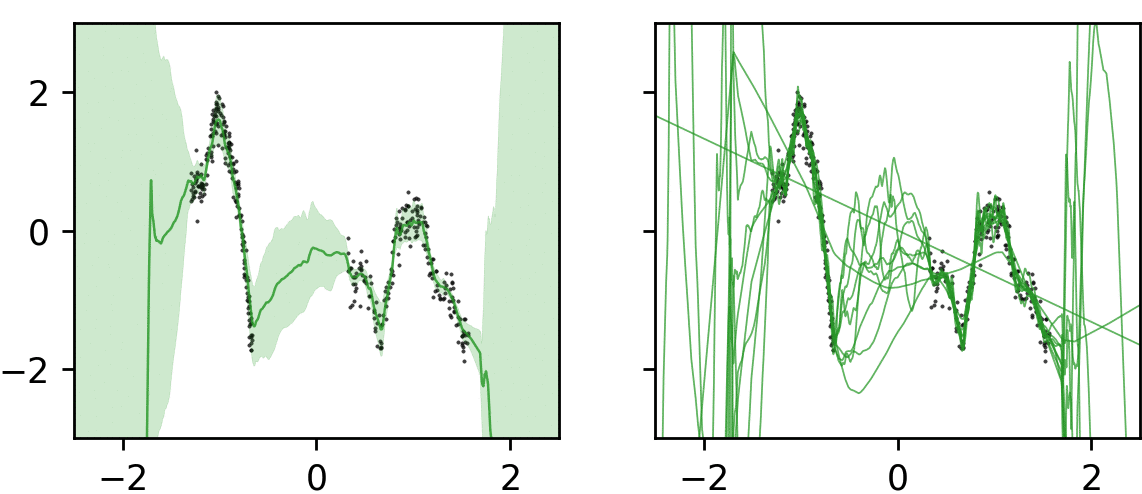
\includegraphics[scale=.35]{figures/antoran.png}
\caption{Toy regression problem using a deep ensemble. Right panel shows individual DNN prediction functions. Left panel gives the estimated epistemic uncertainty of the deep ensemble. Figure from \citet{antoran_depth_2020}.}
\label{fig:epinet}       % Give a unique label
\end{figure}

Deep ensembles are made up of an ensemble of individual DNNs, each trained independently on the same dataset to predict the desired output features. Different random initializations of the same NN at the start of training leads to widely different prediction functions \citep{fort_deep_2019}. Deep ensembles exploit this property by incorporating the results of many differently initialized NNs, increasing the diversity of predictors. This not only yields higher prediction accuracy, but also allows for state-of-the-art aleatoric and epistemic uncertainty quantification \citep{ovadia_can_2019, gustafsson_evaluating_2020}.

To model the aleatoric uncertainty in a regression task, each individual DNN composing the ensemble is trained to minimize the following negative log-likelihood loss function over all training examples $i$ \citep{lakshminarayanan_simple_2017}
\begin{equation}
    L(y_i\mid\mathbf{x}_i) = \frac{{\rm log}(\hat{\sigma}^2(\mathbf{x}_i))}{2} + \frac{\|y_i - \hat{y}(\mathbf{x}_i)\|_2^2}{2\hat{\sigma}^2(\mathbf{x}_i)}.
\end{equation}
The DNN predicts the aleatoric uncertainty $\hat{\sigma}_a$ for each example prediction, as well as the example label $\hat{y}$ as in standard DNN regression, eq.~\ref{eqn:egloss}. This form of loss function assumes the aleatoric error has a Gaussian distribution, usually a reasonable approximation. In practice the DNNs are trained to predict the log variance $\hat{s}(\mathbf{x}_i) = {\rm log}(\hat{\sigma}^2(\mathbf{x}_i))$
\begin{equation}
\label{eqn:log_loss}
    L(y_i\mid\mathbf{x}_i) = \frac{\hat{s}(\mathbf{x}_i)}{2} + \frac{e^{-\hat{s}(\mathbf{x}_i)}\|y_i - \hat{y}(\mathbf{x}_i)\|_2^2}{2}
\end{equation}
since this is more numerically stable \citep{kendall_what_2017}.

During model prediction, predictions from all DNNs composing the ensemble are combined. The final predicted label is the mean over the ensemble predictions. For an ensemble with $M$ DNNs $\hat{y}(\mathbf{x}) = (1/M)\sum_{j=1}^M \hat{y}^j(\mathbf{x})$. Similarly, the final aleatoric uncertainty is given by $\hat{\sigma}^2_a(\mathbf{x}) = (1/M)\sum_{j=1}^M \hat{\sigma}_a^2(\mathbf{x})^j$.
The variance of the label predictions $\hat{y}^j$ over the ensemble is used to model the epistemic uncertainty, resulting in total predicted uncertainty
\begin{equation}
\begin{aligned}
    \hat{\sigma}^2(\mathbf{x}) &= \hat{\sigma}^2_a + \hat{\sigma}^2_e \\
    \hat{\sigma}^2(\mathbf{x}) &= \frac{1}{M}\sum_{j=1}^M \hat{\sigma}_a^2(\mathbf{x})^j + \frac{1}{M}\sum_{j=1}^M\Big[\hat{y}^j(\mathbf{x})  - \frac{1}{M}\sum_{j=1}^M \hat{y}^j(\mathbf{x})\Big]^2.
\end{aligned}
\end{equation}
Very few DNNs are needed in the ensemble, $M \approx 5 - 10$, for the method to achieve state-of-the-art uncertainty quantification \citep{lakshminarayanan_simple_2017}. Figure \ref{fig:epinet} visualizes the epistemic uncertainty prediction for a toy regression problem. In the area far from the training examples, the DNNs composing the ensemble strongly disagree in their predictions, giving a high epistemic uncertainty.

In multitask problems, the aleatoric uncertainties can actually replace the hyperparameters that determine the relative importance of individual tasks in the loss function \citep{kendall_multi-task_2018}. The DNNs automatically tune their own hyperparameters by learning the aleatoric uncertainties during training. 

\subsection{Simulation-Based Inference (SBI)}


\subsection{Blazars}
Blazars are active galactic nuclei whose powerful relativistic jets point at small angle $\theta_{\rm obs}$  to the Earth line-of-sight \citep{urry_unified_1995}, so that the Doppler-boosted jet emission dominates the observed spectral energy distribution (SED). This SED is characterized by a low energy peak caused by synchrotron radiation from energetic electrons, and a high energy peak generally attributed to Inverse Compton scattering of photons by these same electrons \citep{maraschi_jet_1992}. The seed photons can either be from the synchrotron emission (SSC) or from an external source such as the accretion disk or broad line region (EC). The sources are further subdivided by the frequency of the $\nu F_\nu$ synchrotron peak \citep{abdo_spectral_2010}, with ${\rm log}\,\nu_{\rm sy} <14$ labeled LBL (Low peak BL Lacs, and most Flat spectrum Radio Quasars FSRQ) and ${\rm log}\,\nu_{\rm sy} > 15$ called HBL (High peak BL Lacs). Here the frequency is in Hz, and IBL represent the intermediate case. We have yet to determine how the jets are energized and launched with bulk Lorentz factor $\Gamma$, but an attractive origin is the \citet{blandford_electromagnetic_1977} process, so that the jet axis may be associated with the spin axis of the central black hole and the angular momentum axis of the surrounding accretion disk. The jet $e^+/e^-$ obtain an energy distribution extending to $\gamma_{\rm max} \sim 10^4$ or higher, often attributed to shock acceleration. Radiation from these particles spiraling in the embedded magnetic field $B$ can be used to constrain the geometry and energetics of the emission zone and, by inference, the jet accelerator.

Blazars are active galactic nuclei whose powerful relativistic jets point at small angle $\theta_{\rm obs}$  to the Earth line-of-sight \citep{urry_unified_1995}, so that the Doppler-boosted jet emission dominates the observed spectral energy distribution (SED). This SED is characterized by a low energy peak caused by synchrotron radiation from energetic electrons, and a high energy peak generally attributed to inverse-Compton (IC) scattering of photons by these same electrons \citep{maraschi_jet_1992}, a.k.a. synchrotron self-Compton (SSC). The seed photons can also originate from an external source such as the accretion disk or broad line region (External Compton, EC). Blazars can be subdivided by the frequency of their synchrotron peak \citep{abdo_spectral_2010} into HSP, LSP and ISP sources. HSP tend to to peak in the X-ray.
We have yet to determine how the jets are energized and launched with bulk Lorentz factor $\Gamma$, but an attractive origin is the \citet{blandford_electromagnetic_1977} process, so that the jet axis may be associated with the spin axis of the central black hole and the angular momentum axis of the surrounding accretion disk. The jet $e^+/e^-$ obtain an energy distribution extending to $\gamma_{\rm max} \sim 10^4$ or higher, often attributed to shock acceleration or magnetic reconnection. Radiation from these particles spiraling in the embedded magnetic field can be used to constrain the geometry and energetics of the emission zone and, by inference, the jet accelerator.

In studying jet geometry polarization can be particularly useful. Radio VLBI studies have long shown that the pc-scale jet can be substantially polarized. Recently much effort has been spent measuring the optical polarization properties of blazars, since this probes even smaller scales, closer to the acceleration zone. This polarization is often quite variable, offering new dynamical information on the jet structure \citep[e.g.][]{blinov_robopol:_2015, lynch_green_2018}.
Soon we hope to measure the X-ray polarization of a number of blazars with \textit{IXPE} \citep{weisskopf_imaging_2016}, probing closer to the jet acceleration zone than ever before.

Recent optical monitoring campaigns have revealed new polarization patterns. In addition to typical stochastic behavior of polarization fraction ($\Pi$) and angle (PA), \citet{blinov_robopol:_2015} found periods of relatively steady rotation of the PA, sometimes extending many $\times \pi$, lasting weeks or months. These rotations are sometimes associated with flares in total intensity and drops in $\Pi$ \citep{blinov_robopol:_2016}. Various models have been proposed to explain this behavior, including a turbulent stochastic model \citep{marscher_turbulent_2014}, a spiraling jet \citep{lyutikov_polarization_2017} and a helical kink propagating along a conical jet \citep{nalewajko_model_2017}. Although these pictures can accommodate multicycle rotations, they fail to address the optical trends found in \citet{blinov_robopol:_2016}.

Blazars are active galactic nuclei whose relativistic jets are oriented at an angle $\theta_{\rm obs}$ within a few degrees, typically $<15^o$ \citep{liodakis_multiwavelength_2018}, from an observer on Earth. This results in the relativistically boosted emission from the jet to outshine the host galaxy. The jet's observed multiwavelength emission, from radio to $\gamma$-rays, is characterized by two broad components. The low-energy component is attributed to synchrotron emission from primary jet electrons, while the high-energy component is still unknown with inverse-Compton (IC) scattering or hadronic processes (proton synchrotron, pion cascades, etc.) as the current favored mechanisms \citep{blandford_relativistic_2019}. 

The characteristic two peaked spectral energy distribution (SED) of blazar jet emission is understood
to consist of a low energy synchrotron peak and a high energy maximum generally attributed to
Compton emission, although in some models models hadronic processes may also contribute to the high
energy flux \citep{boettcher_modeling_2012}. Blazars are often classified by the synchrotron peak frequency
$\rm \nu_{Sy}$, with Low-peak LSP reaching $\rm \nu F_\nu$ maxima in the mm-IR bands, Intermediate ISP sources
peaking in the optical/UV and HSP peaking in the X-rays.
Dramatic variability, on timescales down to minutes in a few cases
\citep{ackermann_minute-timescale_2016}, is another hallmark of blazar emission. While radiation-zone models can reproduce
this general emission pattern, many details remain to be explained and the underlying mechanisms of
jet energization and collimation are still a subject of debate \citep{blandford_relativistic_2018}.


\section{Outline}
\begin{itemize}
\item \S\ref{chap:nn} contains an overview of the data analysis process necessary to go from telescope observations to polarization measurements and energy spectra, including some of the standard pipeline, covered in more detail in the previous chapter.
\item \S\ref{chap:sbi} gives a brief overview of neural network models and the types of deep learning important for X-ray polarimetry, with a discussion of uncertainty quantification for neural networks.
\item \S\ref{chap:nn} describes an application of neural networks to track reconstruction: extracting emission angles, absorption points and photon energies from GPD track images. Comparison of neural network methods to the standard data analysis.
A neural network approach to identifying and removing events outside of the main detector.
\item \S\ref{chap:sbi} illustrates the use of neural network results for polarization estimation: using neural network predicted uncertainties on emission angles to form a proper maximum likelihood estimator of the polarization parameters.
Comparison of neural network methods to the standard data analysis.
Discussion of the impacts of events outside of the main detector gas.
\item \S\ref{chap:conc} contains the conclusion, limitations, and future directions in the field.
\end{itemize}

